\documentclass[conference]{IEEEtran}
\usepackage[T1]{fontenc}
\usepackage{booktabs}
\IEEEoverridecommandlockouts
\usepackage{cite}
\usepackage{amsmath,amssymb,amsfonts}
\usepackage{graphicx}
\usepackage{stfloats}
\usepackage{placeins}
\usepackage{textcomp}
\usepackage{xcolor}
\usepackage{romannum}
\usepackage{array}
\usepackage{url}
\usepackage{float}
\def\BibTeX{{\rm B\kern-.05em{\sc i\kern-.025em b}\kern-.08em
		T\kern-.1667em\lower.7ex\hbox{E}\kern-.125emX}}


\begin{document}

	\author{
		\IEEEauthorblockN{Arpit Kumar, Arpit Bhomia, Ashish Ranjan, Saurav Gupta, and Anand M. Baswade}
		\IEEEauthorblockA{Department of Computer Science and Engineering, Indian Institute of Technology Bhilai, India \\
			Email: \{arpitk, arpitba, ashishr, sauravg, anand\}@iitbhilai.ac.in}}

	\title{TeraMove: Crowd-Aware Physical Relocation of Indoor THz Access Points under Human Blockage}

	\maketitle

	\begin{abstract}
		We present TeraMove, a framework that adapts indoor THz Access Points (APs) to human blockage with a four-tier cascade. The cascade escalates from electronic beam steering to AP height changes and then to full 3D repositioning, and it moves an AP only when lighter adaptations do not provide threshold coverage. TeraMove
		uses spatial human-density context, obtainable from 3D LiDAR, to detect THz link degradation; our evaluation uses a synthetic crowd model.
		TeraMove first establishes an optimal baseline layout for AP placement using a Mixed Integer Linear Programming (MILP) model over 3D
		coordinates and beam orientations.
		Simulations of an indoor floor with synthetic crowds show that crowd-induced
		blockages reduce the coverage of the commissioned layout to about 44.0\%. Beam steering and height changes add only 6.8~pp, because the people around a user block the links from the current APs. Full repositioning with a crowd-aware seed restores coverage to 99.0\% but moves the APs by 83.5~m in total. Over three crowd shifts it keeps coverage at 98.9\%, while a standard PSO without the seed reaches only 59.8\%.
	\end{abstract}

	\begin{IEEEkeywords}
		THz communication, human blockage, access point placement, beam steering, particle swarm optimization, mixed-integer linear programming
	\end{IEEEkeywords}

	\section{Introduction}

	The emergence of 6G networks is driven by applications such as holographic communication, immersive extended reality, and digital twins that demand multi-Terabit-per-second data rates with ultra-low latency. The Terahertz (THz) band (0.1--10~THz), with far more available spectrum than sub-6~GHz and millimeter-wave (mmWave) bands, is widely regarded as an enabling physical layer for 6G. However, THz signals suffer extreme path loss and molecular absorption, requiring narrow, highly directional beams with unobstructed Line-of-Sight (LoS). In populated indoor spaces, a single human crossing the beam can cause attenuation exceeding 20~dB, potentially collapsing the link.

	The straightforward solution is static placement optimization, fixing transmitting nodes at predetermined positions to maximize coverage. Existing methods typically treat this as a 2D problem at a uniform ceiling height. While adequate for an empty floor plan, such deployments assume the environment remains unchanged. However, human mobility continuously changes blockage conditions, and a layout providing near-perfect coverage can degrade as crowds shift.

	3D LiDAR offers a reliable means to capture this changing context. Recent work has demonstrated accurate human tracking and counting indoors using 3D LiDAR \cite{b27,b29}. This spatial human-density information can characterize blockage conditions, while static over-provisioning can lead to unnecessary deployment costs.

	We present \textit{TeraMove}, a context-aware framework that treats transmitting node deployment as a continuous adaptation problem. It uses spatial human-density information to characterize dynamic blockage and first applies a Mixed-Integer Linear Programming (MILP) formulation to minimize the number of transmitting nodes while satisfying coverage and SINR constraints. When coverage falls below a threshold, a 4-tier HPSO framework adapts the network through beam steering, height adjustment, and, when necessary, full 3D repositioning. Under dense crowds Tiers~2 and~3 add little coverage, so most of the gain comes from Tier~4, while a Hungarian algorithm minimizes physical displacement when movement is required.

	Although focused on THz, the framework is transmitter-agnostic and can also apply to mmWave small cells, Wi-Fi APs, and 5G base stations facing dynamic LoS blockages. We use the term ``Access Points'' (APs) throughout for generality.

	The main \textbf{contributions} of this paper are:
	\begin{itemize}
		\item A 4-tier cascade that tries beam steering and height changes before physical repositioning. It shows how much coverage electronic adaptation can recover under crowd blockage (6.8~pp in our evaluation) before AP motion becomes unavoidable, and its Hungarian step cuts the required motion by 20.5\%.

		\item A MILP formulation that jointly optimizes 3D AP placement and azimuth orientation while minimizing the number of APs required to satisfy user-level SINR coverage.

		\item An HPSO algorithm for dynamic repositioning that prioritizes human-density-weighted coverage while penalizing unnecessary displacement.
	\end{itemize}

	\section{Related Work}

	Pedestrian density and mobility strongly affect THz outage and SINR~\cite{b14}, so static deployments are vulnerable to changing human blockage. Existing AP placement methods primarily optimize the network before
	deployment. Baswade~\textit{et al.}~\cite{b4} formulated base-station
	placement using mixed-integer optimization, while Liu~\textit{et al.}~\cite{b7}
	maximized mmWave LoS coverage with multiple APs. Such approaches provide effective initial layouts but do
	not adapt the deployment after propagation conditions change. PSO and
	its variants have also been applied to wireless optimization,
	including 3D UAV-BS placement~\cite{b15} and mmWave massive-MIMO
	beamforming~\cite{b16}. However, these approaches mainly focus on optimizing placement or communication parameters, rather than combining electronic adaptation with physical AP reconfiguration when human blockage changes.
	Physical mobility offers another means of adapting wireless coverage as user locations vary. Wireless platforms based on UAV can adjust their position in three dimensions to improve coverage and optimize their trajectories~\cite{b15,b20}. Similarly, movable APs have been studied for indoor WLANs, where the AP locations are changed according to user distribution~\cite{b21}. Movable antennas further exploit spatial channel variations by dynamically changing antenna positions~\cite{b22}. These approaches do not jointly consider
	indoor THz beam adaptation, vertical AP adjustment, and progressive
	full-3D repositioning based on human blockage.

	Dynamic adaptation also requires information about human
	movement. Vision-based learning has been used to predict impending
	mmWave/THz blockages~\cite{b25}.
	Specifically, 3D LiDAR point clouds have been used for high-resolution indoor crowd counting and geometry tracking~\cite{b27,b29}. These sensing approaches can provide the spatial
	human-density information required for blockage-aware adaptation.

	\section{System Model and Problem Formulation}

	The indoor environment is discretized into a 3D volumetric grid. Let $\mathcal{U}$ denote the set of target user equipment locations requiring coverage, and let $\mathcal{A}$ denote the set of candidate AP locations. Let user $u$ be at $(x_u, y_u, z_u)$ and AP $a$ at $(x_a, y_a, z_a)$, with 3D distance $d_{u,a}$. The user height is fixed at $z_u = 1.0$~m, and the optimization algorithm selects an AP mounting elevation $z_a$ from a discrete set of candidate heights. The floor is divided into $1~\text{m} \times 1~\text{m}$ cells, and each user is placed at the centre of its cell. This channel model serves as the evaluation setting; our contribution is the adaptation mechanism of Section~IV, which does not depend on the details of the model.

	The deterministic line-of-sight path loss combines the Friis free-space loss, molecular absorption \cite{b1,b2} and wall losses:
	\begin{equation}
		\begin{split}
			PL_{\text{LoS}}(u,a) = {} & 20\log_{10}\!\left(\frac{4\pi f d_{u,a}}{c}\right) \\
			& + 4.343\, k(f)\, d_{u,a} + \sum_{w \in \mathcal{W}_{u,a}} L_{w}
		\end{split}
		\label{eq:total_pl}
	\end{equation}
	where $c$ is the speed of light and $k(f)$ is the molecular absorption coefficient. At 300~GHz in indoor air (23~\textdegree C, 10~g/m$^3$ water vapour), ITU-R P.676 gives 6.68~dB/km, i.e., $k(f) = 1.54 \times 10^{-3}$~m$^{-1}$~\cite{itu676}. $\mathcal{W}_{u,a}$ is the set of walls crossed by the segment from $u$ to $a$, and $L_w$ is the material-specific penetration penalty of wall $w$ (e.g., concrete, wood, glass).

	Furthermore, THz signals suffer severe attenuation when occluded by human bodies \cite{b6}. We define an expected dynamic loss based on the normalized human density score $D_h(c) \in [0,1]$ for each grid cell (computed in Section~IV-A) over the set of grid cells $\mathcal{C}_{u,a}$ intersected by the 2D projection of the link, excluding the cells of the AP and of the user. A human only obstructs the signal if the elevation of the beam $z(c)$ as it passes through cell $c$ drops below
	the standard human height $h_{\text{human}}$.
	Using linear interpolation based on the 2D distance $d_{u,c}^{2D}$ from the user to the point of cell $c$ closest to the user and the total 2D distance $d_{u,a}^{2D}$, the lowest beam elevation in cell $c$ is given as:
	\begin{equation}
		z(c) = z_u + \frac{d_{u,c}^{2D}}{d_{u,a}^{2D}} (z_a - z_u)
		\label{eq:beam_height}
	\end{equation}
	The expected dynamic blockage loss is then defined using an indicator function $\mathbb{I}(\cdot)$, which equals 1 if the beam strikes the human body and 0 otherwise:
	\begin{equation}
		L_{\text{dynamic}} = L_{h} \Big[1 - \prod_{c \in \mathcal{C}_{u,a}} \big(1 - D_h(c)\,\mathbb{I}_c\big)\Big]
		\label{eq:dynamic_loss}
	\end{equation}
	where $\mathbb{I}_c = \mathbb{I}\big(z(c) \le h_{\text{human}}\big)$ and $L_{h}$ is the empirical penalty caused by human blockage. The product is the probability that no cell on the path blocks the link, so $L_{\text{dynamic}}$ never exceeds $L_h$.

	We adopt a flat-top sector antenna model parameterized by the half-power beamwidth (HPBW), $\theta_{\text{HPBW}}$, and the AP's mounting azimuth orientation $\phi_a$. Since APs are mounted above users ($z_a > z_u$) with optimal downward tilt, signal gain is calculated only in the horizontal~plane.

	Let $\phi_{u,a}$ be the angle of user $u$ seen from AP $a$, and $\Delta\phi = |(\phi_{u,a} - \phi_a + 180^{\circ}) \bmod 360^{\circ} - 180^{\circ}|$ its deviation from the AP orientation. The transmit gain is:
	\begin{equation}
		G_{\text{tx}}(\Delta\phi) =
		\begin{cases}
			G_{\text{max}}, & \text{if } \Delta\phi \le \frac{\theta_{\text{HPBW}}}{2} \\
			G_{\text{min}}, & \text{otherwise}
		\end{cases}
		\label{eq:beamwidth}
	\end{equation}
	where $G_{\text{min}}$ is practically negligible. A user directly below the AP is treated as inside the main lobe. With the elevation beamwidth fixed, the main-lobe gain scales inversely with $\theta_{\text{HPBW}}$, and a $60^{\circ}$ beam has 30~dBi:
	\begin{equation}
		G_{\text{max}}(\theta_{\text{HPBW}}) = 30 + 10\log_{10}\left(\frac{60^{\circ}}{\theta_{\text{HPBW}}}\right)~\text{dBi}
		\label{eq:gain_bw}
	\end{equation}
	which gives 33.0~dBi at $30^{\circ}$ and 27.0~dBi at $120^{\circ}$. The received power (in W) is
	\begin{equation}
		P_{\text{rx}}^{(u,a)} = 10^{\left(P_{\text{tx}} + G_{\text{tx}}(\Delta\phi) + G_{\text{rx}} - PL_{\text{LoS}} - L_{\text{dynamic}} - 30\right)/10}
	\end{equation}
	where $P_{\text{tx}}$ is transmit power in dBm and $G_{\text{rx}}$ is receive antenna gain. User $u$ is served by AP $a^*(u)$, and its SINR is
	\begin{equation}
		\text{SINR}_u = \frac{P_{\text{rx}}^{(u,a^*)}}{N_0 + \sum_{b \ne a^*} P_{\text{rx}}^{(u,b)}}
		\label{eq:sinr_eval}
	\end{equation}
	The coverage is the density-weighted share of cells that meet the SINR threshold:
	\begin{equation}
		\text{Cov} = \frac{\sum_u D_h(u)\,\mathbb{I}(\text{SINR}_u \ge \text{SINR}_{\text{th}})}{\sum_u D_h(u)}
		\label{eq:coverage}
	\end{equation}
	On an empty floor ($D_h = 0$ everywhere), Cov is the fraction of cells that meet the threshold.

	\section{Proposed Work}

	We place the APs with a MILP (Section~IV-B) and adapt them with a 4-tier HPSO (Section~IV-C) when crowd shifts degrade user coverage below the target.

	\subsection{Context Acquisition from Human-Density Sensing}

	TeraMove uses spatial human-density information to capture changes in the blockage environment. In practice, this contextual data is obtained using 3D LiDAR sensors, which generate real-time topographical point clouds of the room. By subtracting the static background, we isolate dynamic points corresponding to humans or moving furniture. The human density score $D_h(c) \in [0,1]$ for a specific vertical column is calculated as:
	\begin{equation}
		D_h(c) = \min \left(1, \frac{N_{\text{dyn}}(c)}{N_{\text{max}}} \right)
	\end{equation}
	where $N_{\text{dyn}}(c)$ is the number of dynamic LiDAR points detected in the vertical column at cell $c$, and $N_{\text{max}}$ is the expected maximum number of points for a single human body. In our evaluation, we generate the equivalent human-density map with a synthetic crowd model (Section~V) to evaluate coverage and trigger AP adaptation when needed.

	\subsection{Static Baseline Placement via MILP}

	We formulate the baseline optimization problem as a Mixed-Integer Linear Programming (MILP) model. The primary objective is to minimize the total number of APs deployed, expressed by Eq. \eqref{eq:objective}:
	\begin{equation}
		\min \sum_{a \in \mathcal{A}} W_a
		\label{eq:objective}
	\end{equation}
	where $W_a \in \{0,1\}$ equals 1 if an AP is deployed at location $a$, and 0 otherwise. Let $Y_{u,a} \in \{0,1\}$ denote whether user $u$ is associated with AP $a$. Eq. \eqref{eq:assoc1} ensures that each target sub-region is associated with exactly one deployed AP. Eq. \eqref{eq:assoc2} mandates that a user $u$ can only logically associate with a candidate location $a$ if an AP is physically deployed there.
	\begin{gather}
		\sum_{a \in \mathcal{A}} Y_{u,a} = 1, \quad \forall u \in \mathcal{U}
		\label{eq:assoc1} \\
		Y_{u,a} \le W_a, \quad \forall u \in \mathcal{U}, \forall a \in \mathcal{A}
		\label{eq:assoc2}
	\end{gather}

	In practical deployment scenarios where satisfying 100\% coverage is physically or economically infeasible, Eq. \eqref{eq:assoc1} is relaxed to an inequality ($\sum_{a \in \mathcal{A}} Y_{u,a} \le 1$), and a global coverage constraint is introduced. Let $\eta \in (0,1]$ denote the required proportion that must be served. To strictly enforce this spatial coverage ratio, the total number of successfully associated sub-regions must satisfy the following constraint:
	\begin{equation}
		\sum_{u \in \mathcal{U}} \sum_{a \in \mathcal{A}} Y_{u,a} \ge \eta |\mathcal{U}|
		\label{eq:coverage_constraint}
	\end{equation}

	The next constraint enforces the minimum SINR in each sub-region. For every user--AP pair, the received signal plus a big-M relaxation term must exceed the SINR threshold scaled by the total interference-plus-noise:
	\begin{equation}
		\begin{split}
			P_{\text{rx}}^{(u,a)} + \text{Inf} \cdot (1 - Y_{u,a}) \ge \text{SINR}_{\text{th}} \cdot \left( N_0 + \sum_{\substack{b \in \mathcal{A} \\ b \ne a}} P_{\text{rx}}^{(u,b)} W_b \right), \\
			\quad \forall u \in \mathcal{U}, a \in \mathcal{A}
		\end{split}
		\label{eq:sinr}
	\end{equation}
	When $Y_{u,a}=1$ the big-M term vanishes and the constraint enforces the SINR requirement; when $Y_{u,a}=0$ the large constant $\textit{Inf}$ makes the inequality trivially satisfied, deactivating it for unassociated links \cite{b4}. Because $P_{\text{rx}}^{(u,b)}$ is precomputed for each $(u,b)$ pair and $W_b$ is binary, the entire formulation remains linear and solvable by standard MILP solvers.

	\subsection{Dynamic AP Repositioning via HPSO}

	While MILP optimizes static deployments, indoor crowds are dynamic. To
	avoid static over-provisioning, we dynamically reposition APs to track
	evolving human densities.

	We achieve this using a Hierarchical Particle Swarm Optimization (HPSO)
	algorithm based on \cite{b11,b13}, which activates search dimensions in
	tiers. Each particle updates its position $x_i$ (encoding AP parameters)
	and velocity $v_i$ over $T$ iterations:
	\begin{equation}
		v_i^{(t+1)} = w \cdot v_i^{(t)} + c_1 r_1 (p_i^{\text{best}} -
		x_i^{(t)}) + c_2 r_2 (g^{\text{best}} - x_i^{(t)})
		\label{eq:pso_velocity}
	\end{equation}
	where inertia weight $w$ decreases linearly from $0.9$ towards $0.4$; $c_1 = c_2
	= 1.5$; $r_1, r_2 \sim U(0,1)$; and $p_i^{\text{best}}$ and
	$g^{\text{best}}$ denote personal and global bests. Positions update as
	$x_i^{(t+1)} = x_i^{(t)} + v_i^{(t+1)}$ with velocity clamping, and $z_a$, $\phi_a$ and $\theta_{\text{HPBW}}$ are rounded to the candidate values of Table~\ref{tab:sim_params}.

	The swarm's composite fitness function is:
	\begin{equation}
		F = w_c \cdot R_{\text{cell}} + w_d \cdot R_{\text{density}} + B -
		\beta \cdot M - \gamma \cdot C_p
		\label{eq:fitness}
	\end{equation}
	where $R_{\text{cell}}$ is the proportion of cells meeting the SINR
	threshold, $R_{\text{density}}$ is the covered human density ratio (the coverage defined in Section~III), $B = 0.5$ is
	a target-coverage bonus added when $R_{\text{density}} \ge 0.9$ ($B = 0$ otherwise), and $M$ penalizes physical displacement:
	\begin{equation}
		M = \frac{1}{n\sqrt{L^2 + W^2 + H^2}} \sum_{i=1}^{n} \|r_i - r_i^{\text{prev}}\|
		\label{eq:movement}
	\end{equation}
	where $r_i^{\text{prev}}$ is the position of AP $i$ before adaptation and $L \times W \times H$ is the building size. Note that $D_h$ has two roles: it is the occlusion probability in~\eqref{eq:dynamic_loss} and the demand weight in $R_{\text{density}}$. $C_p$
	prevents APs from clustering too closely:
	\begin{equation}
		C_p = \frac{1}{n(n-1)} \sum_{i=1}^{n}\sum_{\substack{j=1 \\ j \ne
				i}}^{n} \max\left(0,\ 1 - \frac{\|r_i - r_j\|}{d_{\min}}\right)
		\label{eq:clustering_penalty}
	\end{equation}
	where $n$ is the AP count, $\|r_i - r_j\|$ is the horizontal (2D) distance between APs $i$ and $j$, and $d_{\min}$ is
	the minimum inter-AP spacing. The weights are listed in Table~\ref{tab:sim_params}.

	\subsubsection{4-Tier Cascading Optimization Architecture}

	Since moving APs incurs service interruption and mechanical wear, we introduce a 4-tier cascading optimization architecture that progressively unlocks more degrees of freedom only when simpler adjustments prove insufficient.

	\begin{itemize}
		\item \textbf{Tier 1 (Baseline Evaluation):} If current density-weighted
		coverage meets the target ($\ge 90\%$), no action is taken,
		avoiding unnecessary computation and movement.

		\item \textbf{Tier 2 (Beam Parameter Optimization):} HPSO first
		optimizes only the azimuth ($\phi_a$) and beamwidth ($\theta_{\text{HPBW}}$). These electronic adjustments do not move any AP.

		\item \textbf{Tier 3 (Height Adjustment):} If Tier~2 coverage
		remains insufficient, the optimizer adjusts the mounting height
		($z_a$), which needs a minor Z-axis movement and takes less time and energy than moving the AP horizontally.

		\item \textbf{Tier 4 (Full Spatial Repositioning):} As a last resort,
		horizontal coordinates ($x_a, y_a$) are unlocked for complete 3D relocation.
		To limit displacement, one-third of the swarm starts within $\pm 2$~m of the current APs. One particle starts from a crowd-aware greedy layout: APs are added one at a time from a candidate set (every cell centre, heights 2.0, 2.6 and 3.0~m, all azimuths, beamwidths $60^{\circ}$, $90^{\circ}$ and $120^{\circ}$), each time the AP that adds the most density-weighted coverage under~\eqref{eq:sinr_eval}. The Hungarian step (Section~IV-C2) matches it to the current APs.
	\end{itemize}

	At each tier, the HPSO locks the velocity components of the dimensions not yet activated. One particle starts at the current configuration, so a tier never returns a configuration with lower fitness than its input.

	\subsubsection{Displacement Minimization via Hungarian Algorithm}

	Let $r_1, \ldots, r_n$ be the current AP positions and $r'_1, \ldots, r'_n$ the positions returned by HPSO. The Hungarian algorithm \cite{b12} finds the one-to-one assignment $\sigma^*$ of current APs to new positions with the least total 3D displacement:
	\begin{equation}
		\sigma^* = \arg\min_{\sigma} \sum_{i=1}^{n} \|r_i - r'_{\sigma(i)}\|
		\label{eq:hungarian}
	\end{equation}

	\section{Experimental Setup and Simulation Results}

	For the experimental setup, we considered IIT Bhilai Engineering department layout. A synthetic crowd model generates the human density. A crowd has 9 circular clusters of radius 2~m with random centres, and the density falls linearly from 1 at a cluster centre to 0 at its edge. Each run and each time step draws a new crowd, and every result is the mean over 30 runs with independent random seeds. The simulation parameters are summarized in Table~\ref{tab:sim_params}.

	We set $\text{SINR}_{\text{th}} = 5$~dB. At 300~GHz this threshold leaves enough power for basic connectivity after molecular absorption, wall losses and co-channel interference, consistent with the minimum SINR for low-order modulation in THz feasibility studies \cite{b5}.

	\begin{table}[htbp]
		\centering
		\caption{Simulation Parameters}
		\label{tab:sim_params}
		\resizebox{\columnwidth}{!}{%
			\begin{tabular}{@{} l l @{}}
				\toprule
				\textbf{Parameter} & \textbf{Value} \\
				\midrule
				Environment Dimensions & $32 \text{ m} \times 20 \text{ m} \times 3 \text{ m}$ \\
				Operating Frequency ($f$) & $300 \text{ GHz}$ \\
				Transmit Power ($P_{\text{tx}}$) & $20 \text{ dBm}$ \\
				Main-Lobe Gain ($G_{\text{max}}$) & $30 + 10\log_{10}(60^{\circ}/\theta_{\text{HPBW}})$ dBi \\
				Receive Gain ($G_{\text{rx}}$) & $0 \text{ dBi}$ \\
				Evaluated Beamwidths ($\theta_{\text{HPBW}}$) & $30^{\circ}, 45^{\circ}, 60^{\circ}, 75^{\circ}, 90^{\circ}, 120^{\circ}$ \\
				Azimuth Rotation Increments & $45^{\circ}$ ($\pi/4$ rad, from North) \\
				Evaluated Elevations ($z_a$) & $2.0 \text{ m}$ to $3.0 \text{ m}$ ($0.2 \text{ m}$ step) \\
				SINR Threshold ($\text{SINR}_{\text{th}}$) & $5 \text{ dB}$ \\
				Target Coverage Threshold ($\eta$) & $0.90$ ($90\%$), $0.95$ ($95\%$), $1.0$ ($100\%$) \\
				System Noise Floor ($N_0$) & $-64$ dBm ($-174$ dBm/Hz, 10 GHz, 10 dB NF) \\
				Static Blockage Penalty ($L_w$) & Solid: $30 \text{ dB}$, Wood: $20 \text{ dB}$, Glass: $15 \text{ dB}$ \\
				Static Cubicle/Desk Height & $1.0 \text{ m}$ \\
				Human Blocker Penalty ($L_{h}$) & $20 \text{ dB}$ (height $1.6 \text{ m}$) \\
				Molecular Absorption ($k(f)$) & $1.54 \times 10^{-3} \text{ m}^{-1}$ (6.68 dB/km) \\
				Grid Cell, User Height ($z_u$) & $1 \text{ m} \times 1 \text{ m}$, $1.0 \text{ m}$ \\
				Min.\ AP Spacing ($d_{\min}$) & $3 \text{ m}$ \\
				Fitness ($w_c, w_d, \beta, \gamma, B$) & $0.4, 0.6, 0.25, 0.3, 0.5$ \\
				Swarm Size, Iterations per Tier ($S, T$) & $50, 20$ \\
				AP Actuator Speed & $0.2 \text{ m/s}$ \\
				\bottomrule
			\end{tabular}%
		}
	\end{table}

	\subsection{Static Baseline Deployment}

	We first evaluate the MILP formulation in a static environment using the HiGHS solver. Solving to a 1\% optimality gap, the solver identifies that 14 APs are needed for 100\% coverage at $\text{SINR}_{\text{th}} = 5$~dB. By evaluating candidate elevations in $0.2$~m increments from $2.0$~m to $3.0$~m, the optimization enables APs to transmit above $1.0$~m cubicles, yielding a 20\% higher peak SINR compared to APs at a uniform height. Fig.~\ref{fig:static_heatmap} shows the SINR of this 14-AP layout.

	Raising $\text{SINR}_{\text{th}}$ from $1$~dB to $5$~dB increases the AP count from 9 to 10 for 90\% coverage. Wider beamwidths ($90^{\circ}$--$120^{\circ}$) require only 10 APs for 90\% coverage, whereas narrow beams ($60^{\circ}$--$75^{\circ}$) require 15, since broader beams cover more of the floor from each AP.

	\begin{figure}[t]
		\centering
		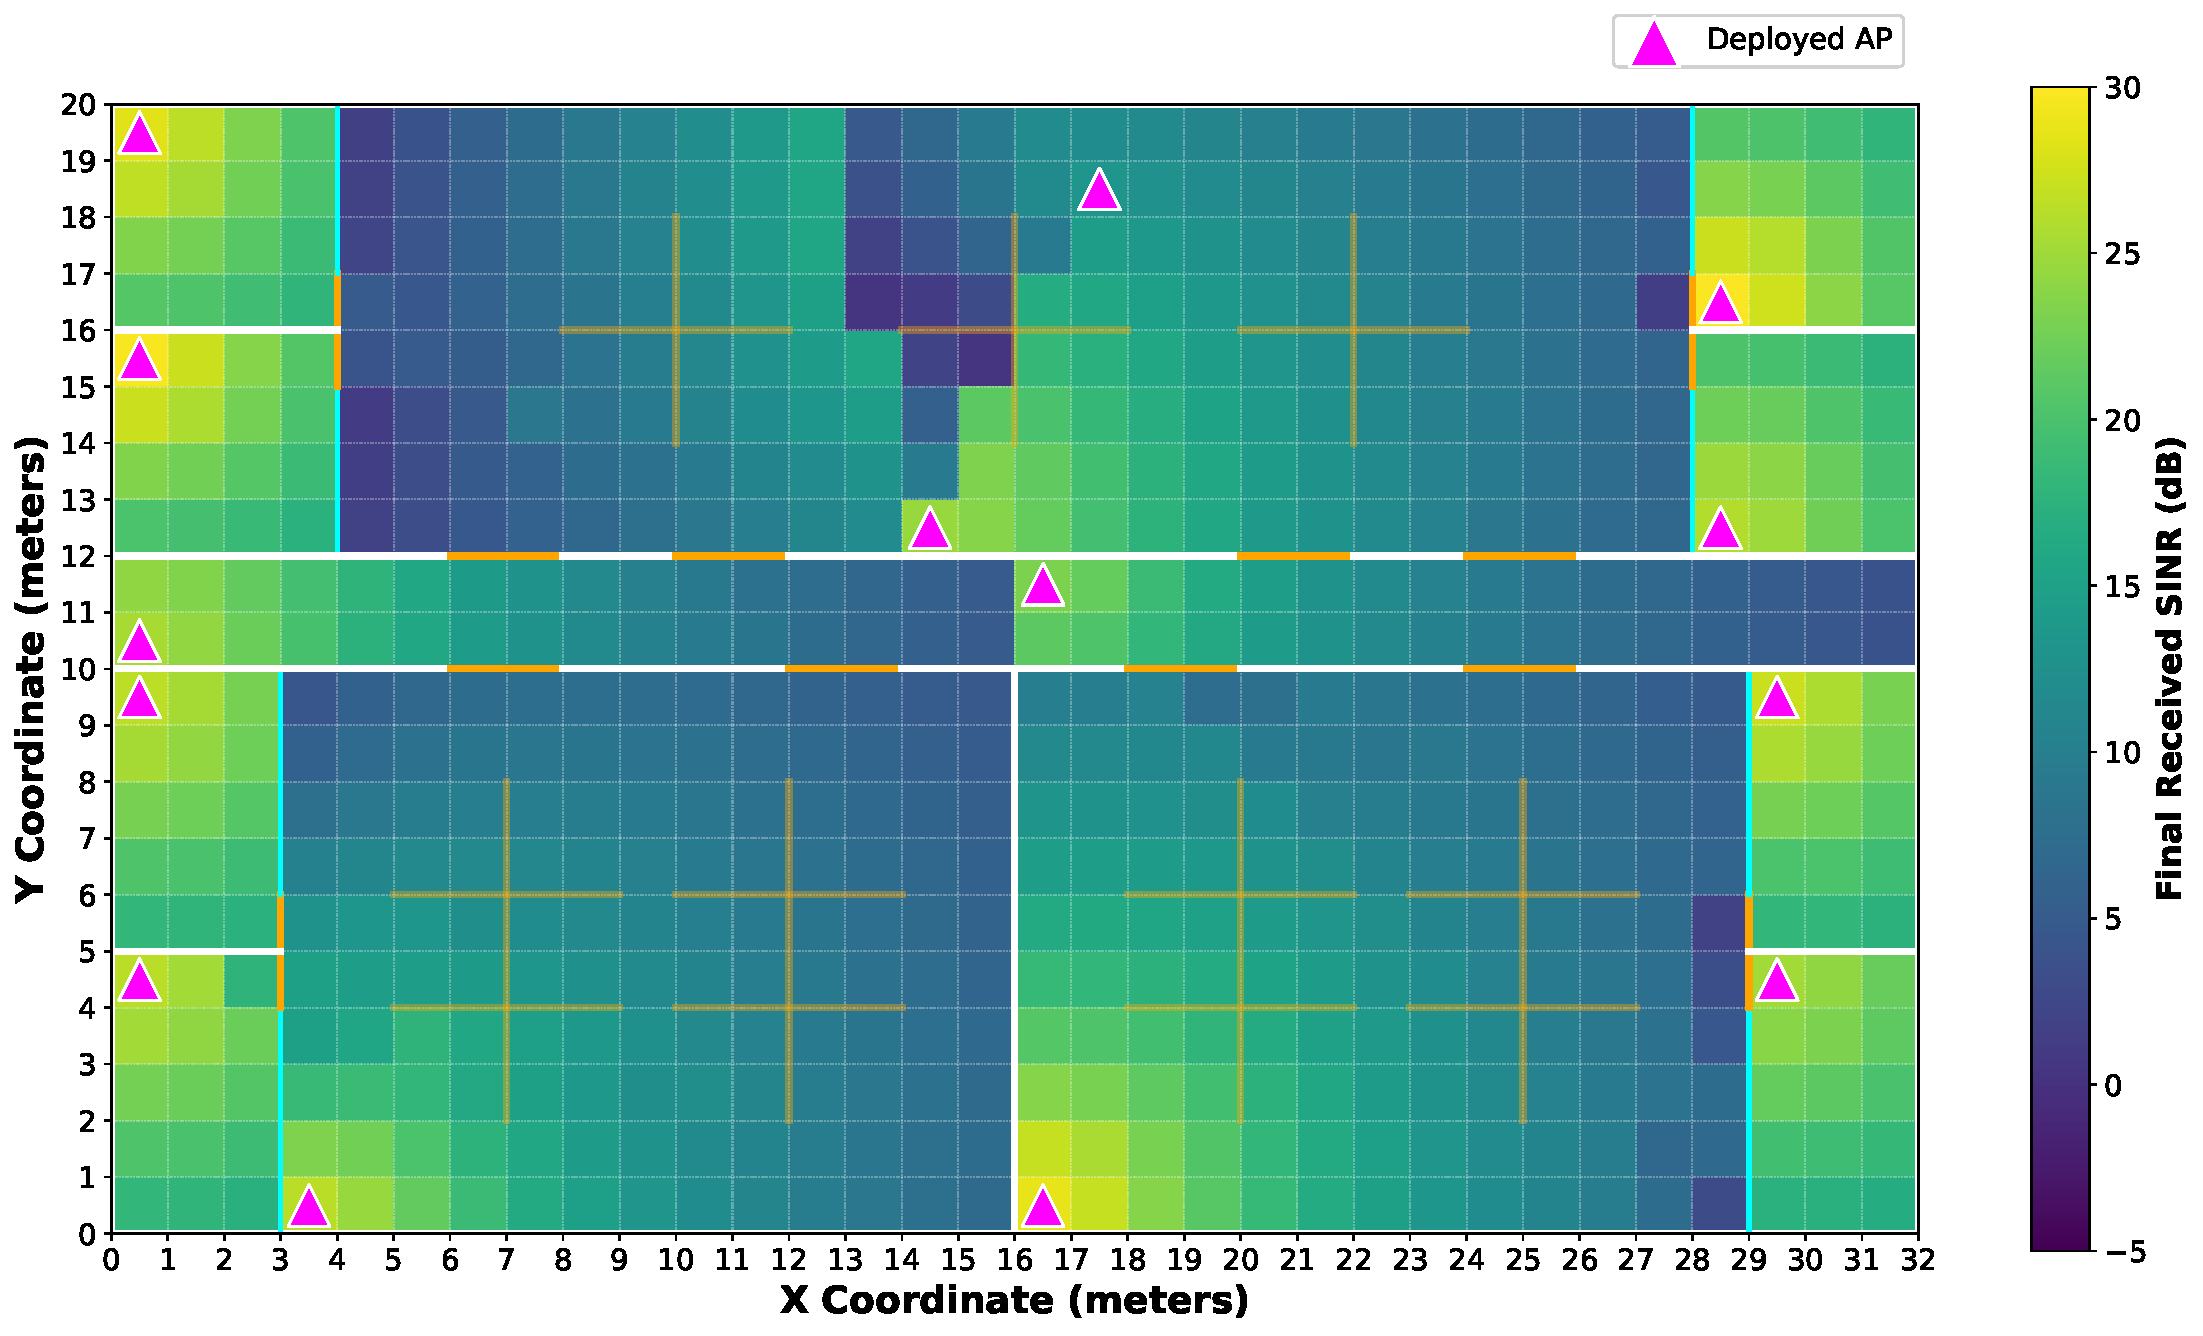
\includegraphics[width=\columnwidth]{APSO_Results_ICC/thz_sinr_heatmap.pdf}
		\vspace{-8pt}
		\caption{SINR distribution of the 14-AP MILP layout.}
		\label{fig:static_heatmap}
		\vspace{-10pt}
	\end{figure}

	\subsection{Tier-wise Coverage and Displacement Analysis}

	The commissioned layout, the starting point of all dynamic runs, keeps the positions of the 14 MILP APs, while the AP heights and beamwidths are not fixed and vary as HPSO requires. The crowd density then causes the coverage loss: human blockage lowers the coverage of this layout to 44.0\% (mean over 30 crowds), and HPSO raises it back to 99.0\%.

	We ran all tiers on every crowd. Table~\ref{tab:tier_summary} summarizes each tier's contribution, with 95\% confidence intervals. From the 14-AP baseline, Tier~2 recovers 4.3~pp (to 48.3\%) without any physical movement ($0.0$~m). Tier~3 adds 2.5~pp for 1.4~m of displacement, and Tier~4 contributes a final 48.2~pp at 83.5~m in total, for a coverage of 99.0\%. Tier~4 meets the 90\% target on 100.0\% of the crowds. Without the body loss, the same layout would cover 97.7\% of these crowds, so the outages come from blockage. By~\eqref{eq:beam_height}, the ray is below head height on the part of the link within $(h_{\text{human}} - z_u)/(z_a - z_u)$ of its length from the user, i.e., 60\% of the link for $z_a = 2.0$~m and 30\% for $z_a = 3.0$~m. The people around a user inside a crowd therefore block the user from the current APs, and only APs moved close to the crowd (Tier~4) restore the link.

	All coverage values assume best-server re-association: each user is served by the strongest AP for the current crowd ($a^*$ in~\eqref{eq:sinr_eval}). This evaluation-time association is separate from the design-time association $Y_{u,a}$ of the MILP. Section~V-D compares it with a layout that keeps the design-time association.

	\begin{table}[htbp]
		\centering
		\caption{Tier-wise Coverage and Displacement Summary (mean $\pm$ 95\% CI over 30 crowds; gain in pp in brackets). Actuation: largest single-AP move at 0.2~m/s (APs move in parallel).}
		\label{tab:tier_summary}
		\resizebox{\columnwidth}{!}{%
			\begin{tabular}{@{} l c c c l @{}}
\toprule
\textbf{Tier} & \textbf{Coverage (\%)} & \textbf{Displ.\ (m)} & \textbf{Actuation (s)} & \textbf{Adjustment Type} \\
\midrule
Baseline & 44.0 $\pm$ 3.2 & 0.0 & 0 & None \\
Tier~2 & 48.3 $\pm$ 3.2 (+4.3) & 0.0 & 0 & Electronic (beam steering) \\
Tier~3 & 50.8 $\pm$ 3.1 (+2.5) & 1.4 & 2.9 & Minor physical (Z-axis) \\
Tier~4 & 99.0 $\pm$ 0.4 (+48.2) & 83.5 & 73.8 & Full 3D repositioning \\
\bottomrule
\end{tabular}%
		}
		\vspace{-10pt}
	\end{table}

	\begin{figure*}[!t]
		\centering
		\begin{minipage}{0.32\textwidth}
			\centering
			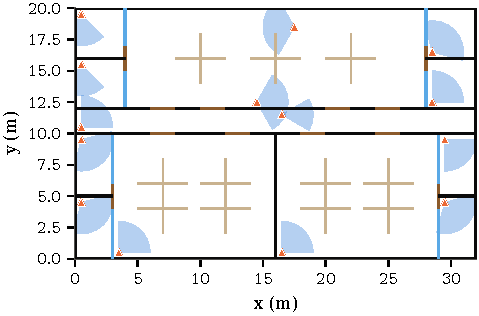
\includegraphics[width=\linewidth]{APSO_Results_ICC/fig2a_aps_before.pdf}
			\vspace{2pt}
			\centerline{\small (a) Step 1: Baseline AP Positions}
			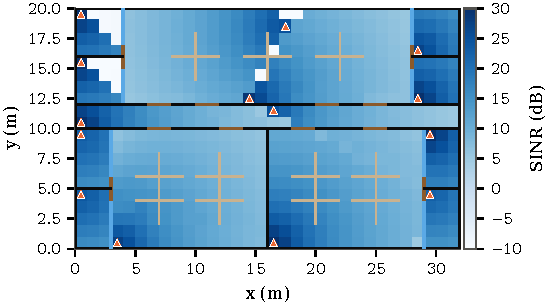
\includegraphics[width=\linewidth]{APSO_Results_ICC/fig2b_sinr_prev.pdf}
			\vspace{2pt}
			\centerline{\small (b) Step 2: Established Stable SINR}
		\end{minipage}\hfill
		\begin{minipage}{0.32\textwidth}
			\centering
			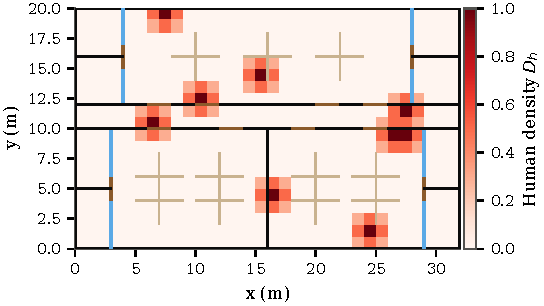
\includegraphics[width=\linewidth]{APSO_Results_ICC/fig2c_density.pdf}
			\vspace{2pt}
			\centerline{\small (c) Step 3: New Human Density Shifts}
			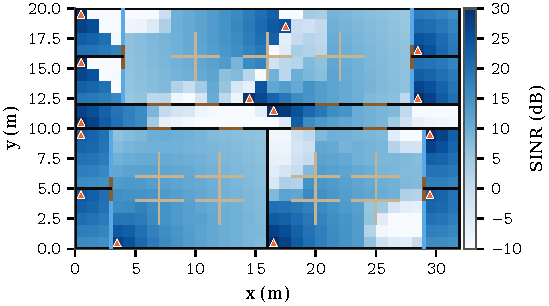
\includegraphics[width=\linewidth]{APSO_Results_ICC/fig2d_sinr_before.pdf}
			\centerline{\small (d) Step 4: Blockage Degrades SINR}
		\end{minipage}\hfill
		\begin{minipage}{0.32\textwidth}
			\centering
			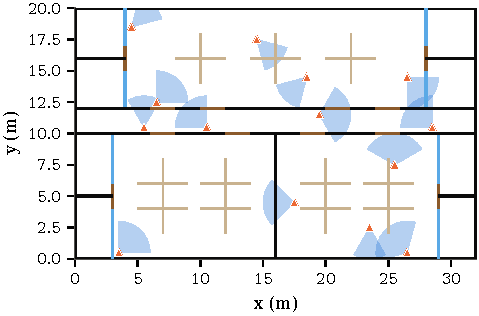
\includegraphics[width=\linewidth]{APSO_Results_ICC/fig2e_aps_after.pdf}
			\centerline{\small (e) Step 5: HPSO Repositions APs}
			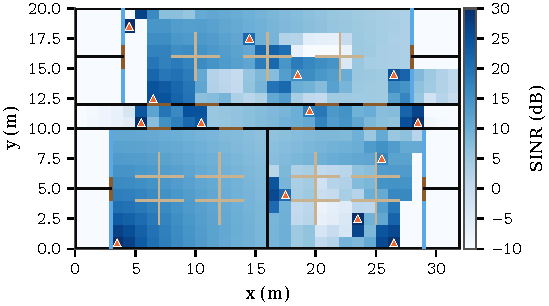
\includegraphics[width=\linewidth]{APSO_Results_ICC/fig2f_sinr_after.pdf}
			\centerline{\small (f) Step 6: SINR After Adaptation}
		\end{minipage}
		\caption{Adaptation sequence at $t_{0}$ for one run: the commissioned layout~(a) gives stable SINR~(b); a crowd shift~(c) degrades it~(d); HPSO re-angles and moves the APs~(e) and raises coverage from 41.2\% to 97.6\%~(f).}
		\label{fig:dynamic_lifecycle_combined}
		\vspace{-12pt}
	\end{figure*}

	Tier~2 gives 7.8\% of the total improvement at zero physical cost, by adjusting beam direction and width through phased-array control. The optimizer takes about 3.6~s for Tier~2 and 66.8~s for Tier~4 on one CPU core. For the moves of Tiers~3 and~4, the Hungarian assignment (Section~IV-C2) replaces a nearest-neighbor matching and reduces the Tier-4 displacement from 105.0~m to 83.5~m, a 20.5\% saving (Wilcoxon $p <0.001$).

	\subsection{Temporal Crowd Adaptation}

	To evaluate robustness under changing crowds, we simulated three consecutive crowd shifts at discrete time steps ($t_0, t_1, t_2$), each drawn independently from the synthetic crowd model. Each step starts from the layout left by the previous step. HPSO raises coverage from 42.7\% to 98.9\% at $t_0$, from 28.5\% to 99.0\% at $t_1$, and from 27.1\% to 98.7\% at $t_2$. The total AP displacement is 87.5~m, 89.2~m and 88.3~m at the three steps. Tiers~2 and~3 do not reach the 90\% target, so the cascade reaches Tier~4 at every step and meets the target in 100.0\% of the steps. Coverage before adaptation is lower at $t_1$ and $t_2$, since the layout from the previous step was placed for a different crowd.

	Fig.~\ref{fig:dynamic_lifecycle_combined} presents the adaptation sequence at $t_{0}$ for one run: from the commissioned AP configuration~(a) and its SINR on the empty floor~(b), a new crowd shift~(c) lowers coverage to 41.2\%~(d), and HPSO re-angles and moves the APs by 75.4~m in total~(e), which raises coverage to 97.6\%~(f).

	\subsection{Comparison with Alternative Approaches}

	We evaluate HPSO against standard Particle Swarm Optimization (PSO) and a Genetic Algorithm (GA). The crowd-aware greedy layout of Tier~4, used alone and matched to the current APs by the Hungarian step, reaches 98.6\% with 107.2~m of movement in the events of Fig.~\ref{fig:coverage_vs_density}. The unconstrained PSO serves as a baseline to isolate the benefits of hierarchical tier constraints; it optimizes the identical composite objective function~\eqref{eq:fitness} (including displacement penalty $\beta M$) but without tier-clamping, updating all 3D coordinates and beam parameters simultaneously. GA serves as a population-based benchmark to verify improvements are not PSO-specific. PSO and GA get no seed and $3T$ iterations, the same worst-case budget as Tiers~2--4. We add three reference arms: the static layout with design-time association, the static layout with re-association, and re-association plus Tier~2 only.

	Fig.~\ref{fig:coverage_vs_density} shows coverage after one adaptation step as human density increases. Coverage falls as the crowd grows for the static arms and the unseeded baselines, while HPSO stays above 95\%. Re-association alone gives the same coverage as the design-time association (44.7\% and 44.7\%), because for 98.9\% of the crowd the design-time AP is still the strongest one. HPSO reaches 97.6\% on average, against 44.7\% for the static layout, and Tier~2 alone reaches 50.2\%. HPSO meets the 90\% target in 99.2\% of the events. Standard PSO and GA reach 62.9\% and 64.5\% (Wilcoxon test against HPSO: $p <0.001$ for both).

	The cascade tries beam steering before physical relocation, but under these crowds Tier~4 is needed in every event. Over the three crowd shifts of Section~V-C, HPSO moves the APs by 265.0~m in total, against 47.0~m for standard PSO and 124.3~m for GA; the extra movement raises mean coverage to 98.9\%, against 59.8\% and 61.5\%. In those runs (9 clusters) the HPSO result equals its greedy seed in every step. In the single-step events of Fig.~\ref{fig:coverage_vs_density}, HPSO moves the APs by 102.4~m on average, against 14.8~m for PSO and 28.8~m for GA. The greedy seed therefore does most of the work: HPSO returns it unchanged in 84.2\% of these events; in the others, mostly at lower crowd levels, the swarm finds layouts with higher fitness than the seed, with less coverage but less movement.

	\begin{figure}[t]
		\centering
		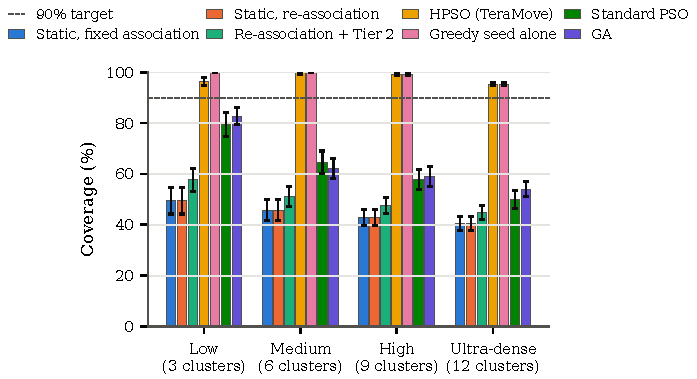
\includegraphics[width=\columnwidth]{APSO_Results_ICC/fig3_coverage_density.pdf}
		\caption{Coverage after one adaptation step for the static layout (fixed association and re-association), re-association with Tier~2, HPSO, the greedy seed alone, standard PSO and GA (mean over 30 crowds per level; error bars: 95\% CI; dashed line: 90\% target).}
		\vspace{-8pt}
		\label{fig:coverage_vs_density}
	\end{figure}

	\section{Discussion}

	TeraMove can run in two modes. In a \textbf{real-time model}, HPSO updates the human-density map from crowd-sensing data such as LiDAR and runs when coverage falls below 90\%. A \textbf{time-based scheduled system} can instead use historical footfall data to estimate density patterns and pre-compute AP configurations for specific times, avoiding continuous sensing. For physical movement, Tier 3 can use linear actuators, while Tier 4 can use ceiling-mounted robotic rails. Flexible PoE cable management keeps the APs connected during movement.

	Practical deployments must account for actuation latency (about 73.8~s for the largest single-AP move in Table~\ref{tab:tier_summary}) and the upfront hardware cost of robotic infrastructure compared to denser static over-provisioning. In our results the coverage target in a crowd is met only by moving APs close to the crowd: Tier~4 moves the APs by 83.5~m in total, against 1.4~m for Tiers~2 and~3.

	\section{Conclusion}

	This paper presents TeraMove for indoor THz AP deployment with moving crowds. A 3D MILP over AP height and beam orientation reduces the required number of APs. Because crowds degrade static layouts, a per-cell human-density score tracks the blockage, and a 4-tier HPSO escalates from beam steering to full 3D repositioning only when lighter tiers fall short. Beam steering and height changes add little in dense crowds, because the people around a user block the links from the current APs. Full repositioning with a crowd-aware seed reaches 98.9\% coverage over three crowd shifts, but it moves the APs by 265.0~m in total. The Hungarian matching cuts the Tier-4 movement by 20.5\% against a nearest-neighbor matching of the APs.

	\begin{thebibliography}{00}
		\bibitem{b1} T. S. Rappaport et al., ``Millimeter Wave Mobile Communications for 5G Cellular: It Will Work!,'' \textit{IEEE Access}, vol. 1, pp. 335--349, 2013.

		\bibitem{b2} Y. Niu et al., ``A survey of millimeter wave communications (mmWave) for 5G: opportunities and challenges,'' \textit{Wireless Netw.}, vol. 21, pp. 2657--2676, 2015.

	\bibitem{b4}
	A. M. Baswade, S. Kiran M. R., B. R. Tamma, and A. Franklin,
	``On Placement of LAA/LTE-U Base Stations in Heterogeneous Wireless Networks,'' in \textit{Proc. ICDCN}, 2018, pp. 37:1--37:10.

		\bibitem{itu676} ITU-R, ``Attenuation by atmospheric gases and related effects,'' Recommendation ITU-R P.676-13, Aug. 2022.

		\bibitem{b5} I. F. Akyildiz, J. M. Jornet, and C. Han, ``Terahertz band: Next frontier for wireless communications,'' \textit{Phys. Commun.}, vol. 12, pp. 16--32, 2014.

		\bibitem{b6}
		B. A. Bilgin, H. Ramezani, and O. B. Akan,
		``Human Blockage Model for Indoor Terahertz Band Communication,''
		in \textit{Proc. IEEE ICC Workshops},
		2019, pp. 1--6.

		\bibitem{b7}
		Y. Liu, Y. Jian, R. Sivakumar, and D. M. Blough,
		``Maximizing Line-of-Sight Coverage for mmWave Wireless LANs With
		Multiple Access Points,'' \textit{IEEE/ACM Trans. Netw.}, vol. 30,
		no. 2, pp. 698--716, 2022.

		\bibitem{b11} J. Kennedy and R. Eberhart, ``Particle swarm optimization,'' in \textit{Proc. IEEE ICNN}, 1995, vol. 4, pp. 1942--1948.

		\bibitem{b12} H. W. Kuhn, ``The Hungarian method for the assignment problem,'' \textit{Naval Res. Logist. Q.}, vol. 2, no. 1--2, pp. 83--97, 1955.

		\bibitem{b13} Y. Shi and R. Eberhart, ``A modified particle swarm optimizer,'' in \textit{Proc. IEEE ICEC}, 1998, pp. 69--73.

		\bibitem{b14}
		V. Petrov, M. Komarov, D. Moltchanov, J. M. Jornet, and
		Y. Koucheryavy, ``Interference and SINR in Millimeter Wave and
		Terahertz Communication Systems With Blocking and Directional
		Antennas,'' \textit{IEEE Trans. Wireless Commun.}, vol.~16, no.~3,
		pp.~1791--1808, 2017.

		\bibitem{b15}
		M. Alzenad, A. El-Keyi, F. Lagum, and H. Yanikomeroglu,
		``3-D Placement of an Unmanned Aerial Vehicle Base Station (UAV-BS)
		for Energy-Efficient Maximal Coverage,'' \textit{IEEE Wireless
			Commun. Lett.}, vol.~6, no.~4, pp.~434--437, 2017.

		\bibitem{b16}
		T. A. Kareem, M. A. Hussain, and M. K. Jabbar,
		``Particle Swarm Optimization Based Beamforming in Massive MIMO
		Systems,'' \textit{Int. J. Interact. Mob. Technol.}, vol.~14,
		no.~5, pp.~176--192, 2020.

		\bibitem{b20}
		M. Tatar Mamaghani and Y. Hong, ``Terahertz Meets Untrusted UAV-Relaying:
		Minimum Secrecy Energy Efficiency Maximization via Trajectory and
		Communication Co-Design,'' \textit{IEEE Trans. Veh. Technol.},
		vol.~71, no.~5, pp.~4991--5006, 2022.

		\bibitem{b21}
		T. Murakami, S. Oka, Y. Takatori, M. Mizoguchi, and F. Maehara,
		``On the Feasibility of an Adaptive Movable Access Point System in a
		Static Indoor WLAN Environment,'' \textit{IEICE Trans. Commun.},
		vol.~E101-B, no.~7, pp.~1693--1700, 2018.

		\bibitem{b22}
		L. Zhu, W. Ma, and R. Zhang, ``Movable Antennas for Wireless
		Communication: Opportunities and Challenges,'' \textit{IEEE Commun.
			Mag.}, vol.~62, no.~6, pp.~114--120, 2024.

		\bibitem{b25}
		G. Charan, M. Alrabeiah, and A. Alkhateeb, ``Vision-Aided 6G
		Wireless Communications: Blockage Prediction and Proactive Handoff,''
		\textit{IEEE Trans. Veh. Technol.}, vol.~70, no.~10,
		pp.~10193--10208, 2021.
		\bibitem{b27}
		J.-S. Yoon, S.-H. Bae, and T.-Y. Kuc, ``Human Recognition and Tracking in Narrow Indoor Environment using 3D Lidar Sensor,'' in \textit{Proc. ICCAS}, 2020, pp. 978--981.

		\bibitem{b29}
		C. Romero-Gonz\'alez \textit{et al.}, ``InLiDa: A 3D Lidar Dataset for People Detection and Tracking in Indoor Environments,'' in \textit{Proc. VISAPP}, 2017, pp. 484--491.

	\end{thebibliography}

\end{document}

